\documentclass[letterpaper]{article}
\usepackage{spconf,amsmath,amssymb,graphicx}
\usepackage[hidelinks]{hyperref}

\usepackage{subcaption}
\usepackage{tikz}
\usetikzlibrary{arrows.meta}
\usetikzlibrary{positioning}
\usetikzlibrary{arrows}

\usepackage{algorithm}
\usepackage{algpseudocode}
\usepackage{listings}
\usepackage{xcolor}
\usepackage{booktabs}
\usepackage{enumitem}

\newcommand{\R}[0]{\mathbb{R}}
\newcommand{\N}[0]{\mathbb{N}}
\newcommand{\C}[0]{\mathbb{C}}
\newcommand{\bigoh}{\mathcal O}

\newcommand{\mypar}[1]{{\bf #1.}}

\title{Efficient Parallelization of Bor\r{u}vka's \linebreak Minimum Spanning Tree Algorithm}

\fiveauthorsalt
  {\normalsize Samuel Anzalone \\[-0.8ex] {\small BS Computational Science} \\[-0.8ex] {\small \texttt{ansamuel@ethz.ch}}}
  {\normalsize Mike Marti \\[-0.8ex] {\small MS Computer Science} \\[-0.8ex] {\small \texttt{mikmarti@ethz.ch}}}
  {\normalsize Matteo Kamm \\[-0.8ex] {\small MS Computer Science} \\[-0.8ex] {\small \texttt{matkamm@ethz.ch}}}
  {\normalsize Hulda L.\ Hannesdóttir \\[-0.8ex] {\small MS Computer Science} \\[-0.8ex] {\small \texttt{hhannesdo@ethz.ch}}}
  {\normalsize \v{S}imon Hrabec \\[-0.8ex] {\small MS Computer Science} \\[-0.8ex] {\small \texttt{shrabec@ethz.ch}}}

\begin{document}

\maketitle

\begin{abstract}
% Describe in concise words what you do, why you do it (not necessarily
% in this order), and the main result.  The abstract has to be
% self-contained and readable for a person in the general area. You
% should write the abstract last.
Minimum Spanning Tree algorithms are among the most well-known graph algorithms in computer science. They can be used as
part of a large variety of algorithms to compute intermediate results and are applied in numerous scientific fields. As
such, having implementations that can handle large inputs and compute the result in a reasonable amount of time is of
utmost importance. In this paper, we look at a variety of work distribution and merging strategies that can be used to
implement Bor\r{u}vka's MST algorithm. We developed some implementations using a mixture of these strategies. To measure
and compare the performance of these implementations, we performed benchmarks on the RACKlette cluster and used the
Parallel Boost Graph Library as a baseline. Using these strategies, we were able to develop implementations that are up
to $31.5$ times faster compared to the baseline.
\end{abstract}

\section{Introduction}
% Do not start the introduction with the abstract or a slightly modified
% version. It follows a possible structure of the introduction. 
% Note that the structure can be modified, but the
% content should be the same. Introduction and abstract should fill at most the first page, better less.
\label{sec:intro}
In this section we briefly introduce and explain what Minimum-Spanning-Tree algorithms are used for. In addition, we
describe our contribution to the scientific community as well as work related to ours.

Formally, an MST of a given undirected connected graph $G = (V, E)$ with vertices $V = \{ 0, \dotsc, n - 1 \}$ and
weighted edges $E \subseteq V \times V$, can be defined as an ayclic subgraph of $G$ which connnects all vertices in
$V$ with the least total weight.

\mypar{Motivation}
% The first task is to motivate what you do.  You can
% start general and zoom in one the specific problem you consider.  In
% the process you should have explained to the reader: what you are doing,
% why you are doing, why it is important (order is usually reversed).
%
% For example, if my result is the fastest sorting implementation ever, one
% could roughly go as follows. First explain why sorting is important
% (used everywhere with a few examples) and why performance matters (large datasets,
% realtime). Then explain that fast implementations are very hard and
% expensive to get (memory hierarchy, vector, parallel). 
%
% Now you state what you do in this paper. In our example: 
% presenting a sorting implementation that is
% faster for some sizes as all the other ones.
The MST problem is one of the most studied problems in combinatorial optimization \cite{graham1985history}. Although the
problem is rather simple, its solutions are often used as part of other algorithms to compute intermediate results.
Other scientific fields, such as epidemiology or taxonomy, apply MST algorithms as can be seen in the following list of
example problems.
\begin{itemize}[noitemsep]
  \item \textbf{Networking} MST algorithms find trees in computer networks that can be used for broadcasting without
    loops \cite{reverse_path_broadcast}.
  \item \textbf{$\frac{3}{2}$-ap\-prox\-i\-mate metric TSP} By combining algorithms that find MSTs, matchings and
    eulerian circuits, one can develop a $\frac{3}{2}$-ap\-prox\-i\-mation algorithm solving the metric traveling
    salesperson problem \cite{christofides1976worst}.
  \item \textbf{Molecular Epidemiology} Minimum-Spanning-Trees are used in molecular epidemiology research to estimate
    relationships among individual strains or isolates \cite{spada2004use, salipante2011inadequacies}.
  \item \textbf{Machine Learning} MSTs are used as part of machine learning algorithms. For example, MSTs can reduce the
    fraction of incorrectly labeled samples when performing brain MRI tissue classification \cite{cocosco2003fully}.
\end{itemize}
For most of these use cases, the speed of the MST algorithm is of great importance e.g. to get quick medical results and
be able to treat the patient accordingly.

\mypar{Contribution}
In our research, we focus on the MST algorithm proposed by Bor\r{u}vka \cite{boruuvka1926jistem, nevsetvril2001otakar},
which is one of the most prominent MST algorithms as of today. We implement this algorithm using different work
distribution and merging strategies. Our implementations use the Message Passing Interface (MPI) for communication.
Randomly generated Kronecker graphs are used to evaluate the performance of our implementation. In this paper we present
a parallel MST implementation that performs significantly better than a state of the art implementation.

\mypar{Related Work}
% Next, you have to give a brief overview of
% related work. For a report like this, anywhere between 2 and 8
% references. Briefly explain what they do. In the end contrast to what
% you do to make now precisely clear what your contribution is.
As the MST problem is very versatile and can be used in various scientific disciplines, there already is some research
on parallelizing MST algorithms. One such paper \cite{chung1996parallel}, which is also the main inspiration of this
project, evaluates how the performance of Bor\r{u}vka behaves when using different pointer jumping schemes. They also
show that in principle a speedup proportional to the number of processors can be achieved.

Other research limits itself on sufficiently dense \linebreak graphs and presents an algorithm for the bulk synchronous
parallel (BSP) model \cite{dehne1998practical}. Furthermore, a parallelization of the MST algorithm using GPUs is
presented in \cite{de2017parallel}.

Some implementations that can be found make use of wait-free Union-Find data structures \cite{wfuf}. Such data
structures speed-up the merge step of the Vor\r{u}vka algorithm. However, they do not aid in distributing the work over
multiple computing nodes.

Our research is similar to that of Chung and Condon \cite{chung1996parallel}, but differs in the work distribution
strategies applied. Moreover, we also evaluate local merging strategies using Union Find data structures additionally to
the pointer jumping schemes. We do not, however, use the wait-free implementations of those data structures as described
in \cite{wfuf}.

\section{Background}
\label{sec:background}
% Give a short, self-contained summary of necessary
% background information. For example, assume you present an
% implementation of sorting algorithms. You could organize into sorting
% definition, algorithms considered, and asymptotic runtime statements. The goal of the
% background section is to make the paper self-contained for an audience
% as large as possible. As in every section
% you start with a very brief overview of the section. Here it could be as follows: In this section 
% we formally define the sorting problem we consider and introduce the algorithms we use
% including a cost analysis.
%
% \mypar{Sorting}
% Precisely define sorting problem you consider.
%
% \mypar{Sorting algorithms}
% Explain the algorithm you use including their costs.
%
% As an aside, don't talk about "the complexity of the algorithm.'' It's incorrect,
% problems have a complexity, not algorithms.
In this section we formally introduce the MST problem, as well as Bor\r{u}vka's algorithm and different parallelization
strategies used in our implementations.

\mypar{Spanning Tree/Forest}
A spanning tree (forest) is an acyclic (disconnected) subgraph $T = (V_T, E_T)$ of an undirected graph $G = (V_G, E_G)$,
where $V_T = V_G$ and $E_T \subseteq E_G$. It is easy to see, that a spanning tree for a graph $G$ is not necessarily
unique, i.e. there can be more than one spanning tree of a graph. For instance, the fully connected graph $K_3$ has
three spanning trees. For simplicity, we will use the term spanning tree throughout this report even though we might be
working with spanning forests in case $G$ is not connected.

\mypar{Minimum-Spanning-Tree Problem}
In the \linebreak MST problem, every edge $e$ of the input graph $G = (V, E)$ has an associated weight. Formally, there
is a weight function $w : E \to \N$ that is given as input. The goal is to find a spanning tree with a minimum edge
weight sum, i.e. the edge weight of all other spanning trees is at least as large. Just like with a spanning tree, an
MST must not necessarily be unique for a given graph $G$.

\mypar{Bor\r{u}vka's Algorithm}
Bor\r{u}vka's algorithm \cite{boruuvka1926jistem, nevsetvril2001otakar} solves the MST problem as described above.
Algorithm \ref{alg:boruvka} contains a high-level overview of how the algorithm operates. The algorithm terminates as
soon as $T$ is a spanning tree. In case the input graph is not connected, the termination condition has to be slightly
adapted to arrive at a forest. The sequential runtime is $\bigoh(m \log n)$, where $m = |E|$ and $n = |V|$ of the input
graph $G = (V, E)$.

\begin{algorithm}[!t]
  \caption{Bor\r{u}vka's algorithm}
  \label{alg:boruvka}
  \begin{algorithmic}
    \State $T \gets \{ \}$
    \While{$\exists$ more than one connected component}
      \For{each component $c$ in $T$}
        \State $e \gets$ \Call{FindLightestOutgoingEdge}{$c$}
        \State $T \gets T \cup e$
      \EndFor
      \State \Call{MergeComponents}{}
    \EndWhile
    \State \Return $T$
  \end{algorithmic}
\end{algorithm}

\mypar{Union Find Data Structure}
A Union Find data structure stores a partition of a set into disjoint subsets in such a way, that finding the
corresponding set of an element and merging two sets takes $\bigoh(\alpha(n))$ time \cite{efficiency_union_find}. These
operations can be used to describe the connected components in the algorithm \ref{alg:boruvka}. Note that the runtime
achieved here is not on a per-operation basis. Single operations can take longer but the data structure adjusts itself
so that successive operations are faster.

\mypar{Pointer Jumping}
Pointer jumping \cite{jeje1992introduction} (also referred to as path doubling) is a design technique that allows an
algorithm to follow a path using only logarithmic time with respect to the length of the longest path. It does this by
redirecting the parent pointers that describe the path, to point to the parent of the parent for each vertex on the path
simultaneously. This process is then repeated until every vertex points to the root of the path. This gives a $\bigoh(n
\log n)$ runtime, where $n$ describes the amount of vertices on the path. This is superior to simply iteratively fixing
each vertex individually, which has a potential worst case runtime of $\bigoh(n^2)$.

\mypar{Supervertex Pointer Jumping}
Supervertex \linebreak pointer jumping \cite{chung1996parallel} is an extension of pointer jumping that uses randomness
to achieve an expected linear time algorithm. The technique is best explained in the aforementioned paper, but the high
level idea is to select a set of vertices to be supervertices, perform pointer jumping on all non-supervertices, until
they reach a supervertex or a root, let each supervertex point to the next supervertex and repeat the process
recursively on the supervertices. After the recursion, it is sufficient to perform only one more pointer jump for all
non-supervertices.

\mypar{MPI}
The message passing interface \cite{clarke1994mpi} is a standard for developing applications on parallel computing
architectures. It defines library routines for inter-core and inter-system communication. Similar to the
C++ standard, there is no reference implementation but multiple open source projects implementing the standard, such as
MPICH and Open MPI \cite{gabriel2004open}.

\mypar{Kronecker Graphs}
Kronecker graphs are a class of graphs constructed from a small base graph by iteratively applying the Kronecker product
\cite{leskovec2010kronecker}. The Graph500, a rating of supercomputer systems focusing on graph algorithms, uses a
variation of this graph construction for their benchmarks \cite{graph500}.

\begin{figure*}
  \begin{subfigure}{0.33\textwidth}
    \centering
    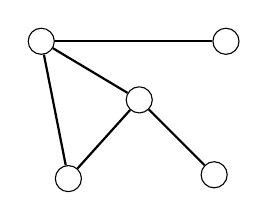
\begin{tikzpicture}[every node/.style={circle,draw,align=center,font=\small,minimum size=.7em},
      node distance=3cm]
      \node (v1) {};
      \node[below right=1.5cm and .1cm of v1] (v2) {};
      \node[below right=.5cm and 1cm of v1] (v3) {};
      \node[below right=1cm of v3] (v4) {};
      \node[right=2cm of v1] (v5) {};
      \path[>={Stealth[black]}, every edge/.style={draw=black, thick}]
        (v1) edge (v2)
        (v1) edge (v3)
        (v1) edge (v5)
        (v2) edge (v3)
        (v3) edge (v4);
    \end{tikzpicture}
    \caption{Original input graph}
    \label{fig:work_distribution_original_input_graph}
  \end{subfigure}
  \begin{subfigure}{0.33\textwidth}
    \centering
    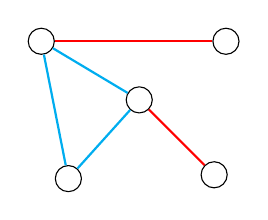
\begin{tikzpicture}[every node/.style={circle,draw,align=center,font=\small,minimum size=.7em},
      node distance=3cm]
      \node (v1) {};
      \node[below right=1.5cm and .1cm of v1] (v2) {};
      \node[below right=.5cm and 1cm of v1] (v3) {};
      \node[below right=1cm of v3] (v4) {};
      \node[right=2cm of v1] (v5) {};
      \path[>={Stealth[black]}, every edge/.style={draw=black, thick}]
        (v1) edge[cyan] (v2)
        (v1) edge[cyan] (v3)
        (v1) edge[red] (v5)
        (v2) edge[cyan] (v3)
        (v3) edge[red] (v4);
    \end{tikzpicture}
    \caption{Edge distributed input graph}
    \label{fig:work_distribution_edge_distributed_graph}
  \end{subfigure}
  \begin{subfigure}{0.33\textwidth}
    \centering
    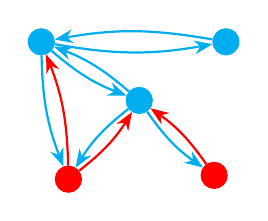
\begin{tikzpicture}[every node/.style={circle,draw,align=center,font=\small,minimum size=.7em},
      node distance=3cm]
      \node[cyan, fill=cyan] (v1) {};
      \node[red, fill=red, below right=1.5cm and .1cm of v1] (v2) {};
      \node[cyan, fill=cyan, below right=.5cm and 1cm of v1] (v3) {};
      \node[red, fill=red, below right=1cm of v3] (v4) {};
      \node[cyan, fill=cyan, right=2cm of v1] (v5) {};
      \path[>={Stealth[black]}, every edge/.style={draw=black, thick}]
        [->] [>={Stealth[cyan]}] (v1) edge[cyan, bend right=10] (v2)
        [->] [>={Stealth[red]}] (v2) edge[red, bend right=10] (v1)
        [->] [>={Stealth[cyan]}] (v1) edge[cyan, bend right=10] (v3)
        [->] [>={Stealth[cyan]}] (v3) edge[cyan, bend right=10] (v1)
        [->] [>={Stealth[cyan]}] (v1) edge[cyan, bend right=10] (v5)
        [->] [>={Stealth[cyan]}] (v5) edge[cyan, bend right=10] (v1)
        [->] [>={Stealth[red]}] (v2) edge[red, bend right=10] (v3)
        [->] [>={Stealth[cyan]}] (v3) edge[cyan, bend right=10] (v2)
        [->] [>={Stealth[cyan]}] (v3) edge[cyan, bend right=10] (v4)
        [->] [>={Stealth[red]}] (v4) edge[red, bend right=10] (v3);
    \end{tikzpicture}
    \caption{Vertex distributed input graph}
    \label{fig:work_distribution_vertex_distributed_graph}
  \end{subfigure}
  \caption{Graph distribution example}
  \label{fig:work_distribution}
\end{figure*}

\section{Approach}
\label{sec:approach}
% Now comes the ``beef'' of the report, where you explain what you
% did. Again, organize it in paragraphs with titles. As in every section
% you start with a very brief overview of the section.

% In this section, structure is very important so one can follow the technical content.

% Mention and cite any external resources that you used including libraries or other code.
This section contains information about the different implementations developed, as well as other technical
details, such as distribution strategies, limitations and the benchmarking infrastructure.

\subsection{Distributing the Work}
There are many ways how a graph can be distributed among multiple computation units. The two strategies that we
considered are distributing the edges and distributing the vertices. A combination of the two would also be conceivable,
but was not considered in this project. As these two strategies have different parallelization capabilities, multiple
implementations for both of these approaches were developed. To get a better understanding of how they operate and how
they compare, the following two paragraphs describe them both.

\mypar{Distribution by Edges}
In this approach, the edges of the input graph are distributed evenly among computation units. An illustration of such a
distribution can be seen in Fig. \ref{fig:work_distribution_edge_distributed_graph}. This strategy allows for a uniform
workload distribution, as every computation unit has the same amount of edges to process when selecting the minimum
weight outgoing edges. On the other hand, the merging of components cannot be parallelized using this approach. This is
because during the merging step, all vertices of a component have to unanimously agree on a new leader. But since a
vertex is not owned by a computation unit, this cannot be accomplished without additional effort.

\mypar{Distribution by Vertices}
In this approach, the vertices of the input graph are distributed (including their incident edges) among computation
units. An example of such a distribution can be seen in Fig. \ref{fig:work_distribution_vertex_distributed_graph}. One
major disadvantage of this approach is that each edge gets distributed twice because it is not guaranteed that
neighboring vertices are assigned to the same computation unit. Consequently, this strategy requires more time to
distribute the graph. Moreover, the workload of each computation unit is unevenly distributed compared to the edge
distribution strategy. Imagine a scenario, where certain vertices have a higher degree (amount of incident edges) than
others. In that case the computation of the minimum weight outgoing edge of each component takes longer for some
computation units whilst others are idle. However, with this approach the merging of components can be parallelized. 

\subsection{Implementations}
\label{sec:implementations}
For this project we developed various C++ implementations, combining different merging approaches with the two
aforementioned distribution strategies. The following list contains all the combinations realized:
\begin{itemize}[noitemsep]
  \item Edge Distributed, merging via
  { \setlist{nolistsep}
  \begin{itemize}[noitemsep]
     \item Union Find 
     \item Union Find with reduced edges
     \item Pointer Jumping
  \end{itemize} }
  \item Vertex Distributed, merging via
  { \setlist{nolistsep}
  \begin{itemize}[noitemsep]
     \item Union Find 
     \item Iterative Vertex Fixing
     \item Pointer Jumping
     \item Supervertex Pointer Jumping
  \end{itemize}
  }
\end{itemize}
Clearly, this list does not contain every possible combination. Intermediate benchmarking showed that some strategies
were not promising enough to be pursued further.

We are not going to give detailed descriptions for all implementations, as their rough idea should be clear with the
information given in section \ref{sec:background}. The ones that might not be self-explanatory are \emph{Edge
Distributed Union Find with reduced edges} and \emph{Vertex Distributed Iterative Vertex Fixing}. The first one uses
an additional optimization where edges with both endpoints in the same component get skipped over. As this removal costs
additional runtime, we have to be cautious about the impact on performance. The second one uses an iterative fixing of
the vertices, briefly mentioned in the pointer jumping paragraph in section \ref{sec:background}. This approach has a
greater theoretical runtime, but uses far less communication compared to the vertex distributed pointer jumping
implementation. The open question here is, whether the lower runtime guarantee is worth the additional communication.
This is answered in section \ref{sec:results}. In addition, the Union Find implementations use the so-called path
compression strategy when performing \verb|find()| operations and we merge sets by rank during \verb|union()| calls
\cite{intro_to_algos}.

Sequential versions of some merging strategies were also implemented to get a better understanding of how they operate.
However, these sequential algorithms did not serve any additional purpose beyond that.

\mypar{Baseline Implementation}
To get an idea of how well our implementations perform, we decided to use the Parallel Boost Graph Library (BGL)
\cite{bgl} as our baseline. We considered other baseline implementations but came to the conclusion that the Parallel
BGL is the most optimized and well-known library. One promising implementation uses OpenMP which might have led to
uncomparable results since we use MPI \cite{15418}.

\mypar{Kronecker Graph Generator}
\label{par:kronecker_graph_generator}
Initially, we experimented with different kinds of graphs and implemented some generators for them, but ultimately
decided to only use Kronecker graphs to benchmark our implementations. Self-written generators can be error-prone and it
is difficult to efficiently generate large graphs. Therefore, we use the reference implementation of the Graph500
specification that is available on
GitHub\footnote{\url{https://github.com/graph500/graph500/tree/newreference/generator}}. An alternative to this is the
Erdös-Renyi graph generator that is part of the Parallel BGL \cite{bgl}. To get reproducible benchmark results across
all algorithm executions, we seeded the graph generator, so that it always generates the same random graph.

\mypar{Communication}
All implementations use MPI as a communication protocol. Besides send and receive routines used to distribute the graph,
we also use scatter, gather and reduction functionalities. To minimize the cost of communication as much as possible, we
keep the amount of MPI subroutine calls to a minimum. We achieve this by first locally preparing the data and then
sending everything at once. This was used to e.g. more efficiently distribute the incident edges in all vertex
distributed implementations. Instead of sending each edge individually, only one send operation containing all edges is
performed for each computation unit.

\mypar{Limitations}
\label{par:limitation}
So far all implementations don't compute the actual MST, but only its edge weight sum. Moreover, the work has to be
distributed among all computation units evenly, i.e. the amount of edges or vertices must be divisible by the amount of
computation units depending on the distribution strategy. For most implementations, both of these limitations are
straightforward to resolve. This is especially true for the MST tree computation, as the lightest edges are distributed
among the computation units anyway.

\mypar{Correctness}
To verify the correctness of our algorithms, we perform unit tests using Catch2. On top of that, we perform differential
tests with large Kronecker graphs that compare our implementations to the baseline (parallel BGL). To get assurance
during development, we use continuous integration that executes the tests and reports potential failure.

\subsection{Benchmarking Infrastructure}
To ease the benchmarking process, we developed an infrastructure that allows us to parameterize the different
algorithms. The results are obtained using the performance measurement tool LIKWID \cite{treibig2010likwid}. LIKWID uses
hardware counters for its measurements and can be invoked by simply marking the code to be benchmarked. This allows us
to benchmark parts of the algorithms and obtain detailed information to further improve certain functionality.

\section{Experimental Results}
\label{sec:exp}
In this section we go over the benchmarking setup, as well as the results that we measured, including their
interpretation.

\subsection{Experimental Setup}
% Specify the platform (processor, frequency, maybe OS, maybe cache sizes)
% as well as the compiler, version, and flags used. If your work is about performance, 
% I strongly recommend that you play with optimization flags and consider also icc for additional potential speedup.
The benchmarks were executed on the RACKlette cluster \cite{racklette}, setup and maintained by a group of students from
ETH.

\mypar{Hardware}
The RACKlette cluster consists of four identical nodes, each of which has two 64-core AMD EPYC 7742 CPUs running at
2.25GHz with 512GB DDR4 3200MT/s RAM and four Nvidia Tesla V100 GPUs with 32GB GDDR5 VRAM for a total of 512 cores, 2TB
of memory and 16 GPUs. The four nodes are connected using a speedy interconnect from \linebreak Mellanox, namely HDR
ConnectX-6 adapters for a \linebreak 200Gbit/s connection.

\mypar{Work Allocation}
All four cluster nodes were used for the benchmarks. We pinned the CPU cores with the purpose that the amount of used
CPU cores was equal on all nodes. In addition, the cores were chosen such that the amount of cache overlap is minimized.
This allocation strategy should lead to more consistent measurements, as otherwise benchmarks with a low MPI core count
could have an unfair advantage due to less network communication.

\mypar{Software}
All benchmarks were conducted using CentOS Linux release 7.9.2009 (Core) with Linux kernel 3.10.0, the MPI
implementation mvapich2 version 2.3.4 and Parallel BGL version 1.78.0. The code was compiled with GCC version 10.3.0
using the compilation flags
\lstinline[basicstyle=\ttfamily\color{black},identifierstyle=\color{black}]|-mavx -march=native -O3|.

\begin{figure}
  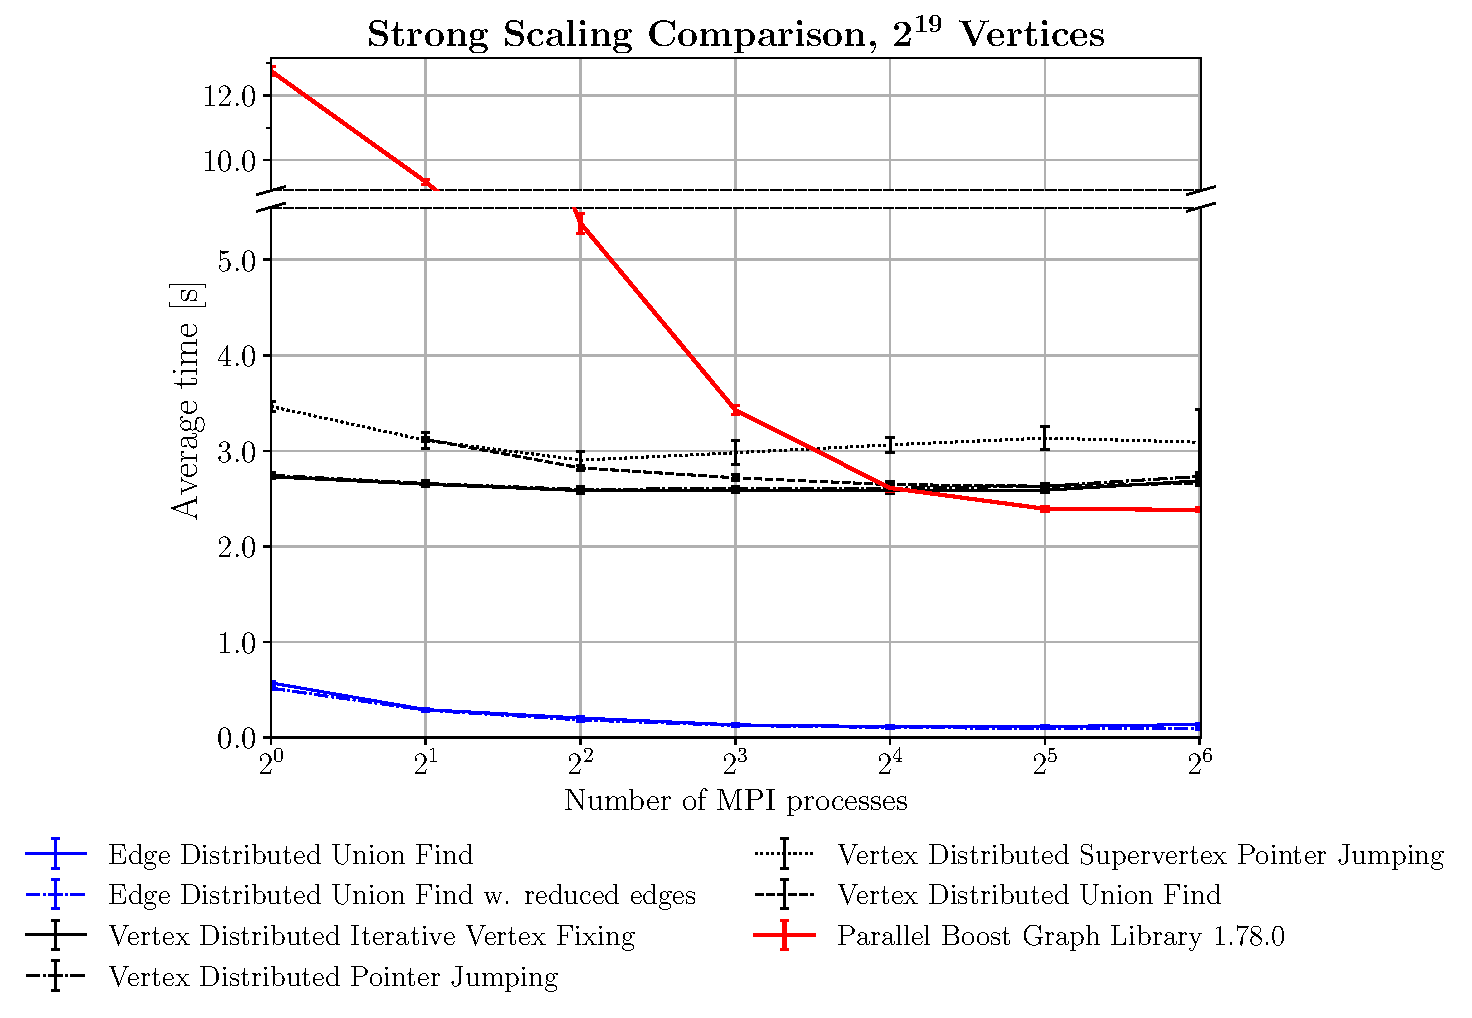
\includegraphics[width=\columnwidth]{../benchmark-results/plots/strongscaling_s19.pdf}
  \caption{Strong scaling comparison with the baseline, $2^{19}$ vertices}
  \label{fig:strongscaling-19}
\end{figure}

\subsection{Performed Benchmarks}
% Then explain what kind of benchmarks you ran. The idea is to give enough information so the experiments are
% reproducible by somebody else on his or her code.
% For sorting you would talk about the input sizes. For a tool that performs NUMA optimization, you would specify the
% programs you ran.
As described in section \ref{par:kronecker_graph_generator}, all benchmarks were performed using Kronecker graphs. These
graphs have $16$ times more edges than vertices (as per Graph500 specification \cite{graph500}). This is to ensure an
average degree of $32$. The implementation \emph{Edge Distributed Pointer Jumping} resulted in bad performance.
Since we are not certain which part of the algorithm causes this, we decided to not include it in our reported
measurements.

\mypar{Baseline Comparison}
To compare our implementations with the baseline, we performed a strong scaling comparison using graphs with $2^{19}$
vertices. The number of MPI processes were the powers of $2$: $2^0, \dotsc, 2^6$. The baseline implementation did not
allow us to go any further than that because the execution took too long. We believe this to be an implementation issue
within the parallel BGL.

\mypar{Implementation Comparison}
To compare our implementations with each other, we performed a strong and weak scaling comparison. The strong scaling
comparison was performed using graphs with $2^{20}$ vertices. The number of MPI processes were the powers of $2$: $2^0,
\dotsc, 2^9$. The weak scaling comparison was performed using the configurations seen on the x-axis of Fig.
\ref{fig:weakscaling}.

\mypar{Detailed Runtime Analysis}
To get a better understanding of which parts of the algorithms require the most runtime, we performed fine-grained
measurements. We differentiated between graph distribution, lightest edge selection and merging. This benchmark was
performed using $64$ MPI processes and a graph with $2^{19}$ vertices.

\mypar{Summarizing Results}
As we are working with runtimes, the arithmetic mean is the obvious choice for summarization. The results for one
algorithm execution were summarized by taking the maximum runtime of any MPI process. To get a summary over all
algorithm iterations, an arithmetic mean was computed. 

\mypar{Repetitions}
We collected measurements until the $90\%$ confidence interval was within $5\%$ of our reported means. This was achieved
by performing $10$ repetitions in all benchmarks, where the first execution is discarded due to warmup.

\subsection{Results}
\label{sec:results}
This section contains the results of the performed benchmarks, including an analysis.
% Next divide the experiments into classes, one paragraph for each. In each class of experiments you typically pursue
% one questions that then is answered by a suitable plot or plots. For example, first you may want to investigate the
% performance behavior with changing input size, then how your code compares to external benchmarks.

% For some tips on benchmarking including how to create a decent viewgraph see pages 22--27 in \cite{Pueschel:10}.

% {\bf Comments:}
% \begin{itemize}
% \item Create very readable, attractive plots (do 1 column, not 2 column plots
% for this report) with readable font size. However, the font size should also
% not be too large; typically it is smaller than the text font size.

% An example is in Fig.~\ref{fftperf} (of course you can have a different style).
% \item Every plot answers a question. You state this question and extract the
% answer from the plot in its discussion.
% \item Every plot should be referenced and discussed.
% \end{itemize}
% 
% \begin{figure}\centering
%   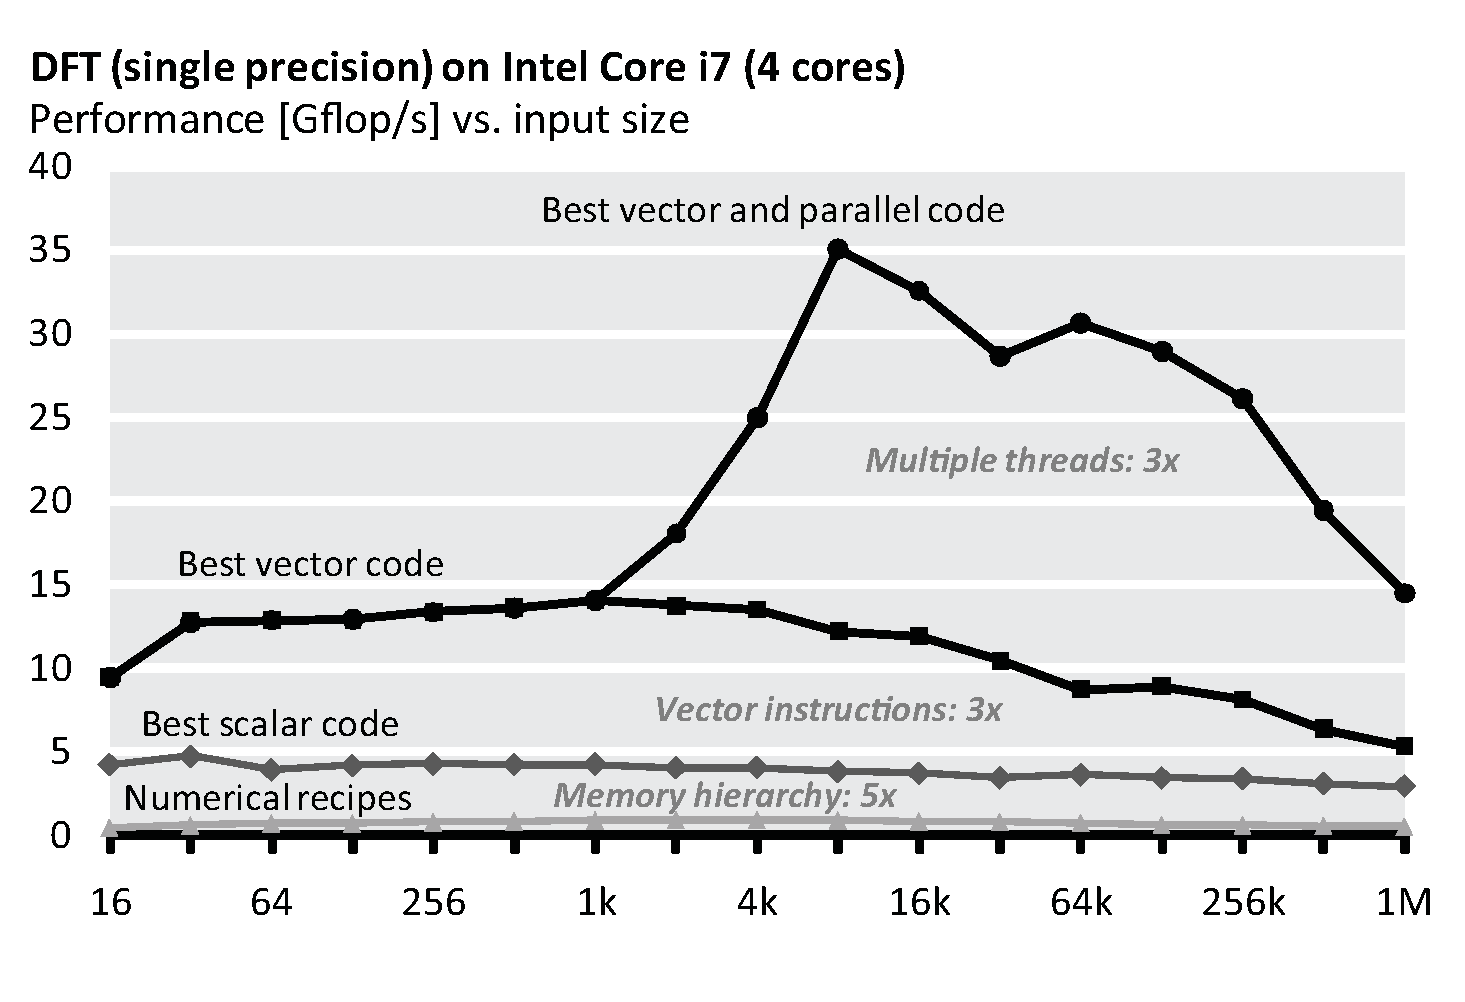
\includegraphics[scale=0.33]{dft-performance.eps}
%   \caption{Performance of four single precision implementations of the
%   discrete Fourier transform. The operations count is roughly the
%   same. The labels in this plot are maybe a little bit too small.\label{fftperf}}
% \end{figure}

\begin{figure}
  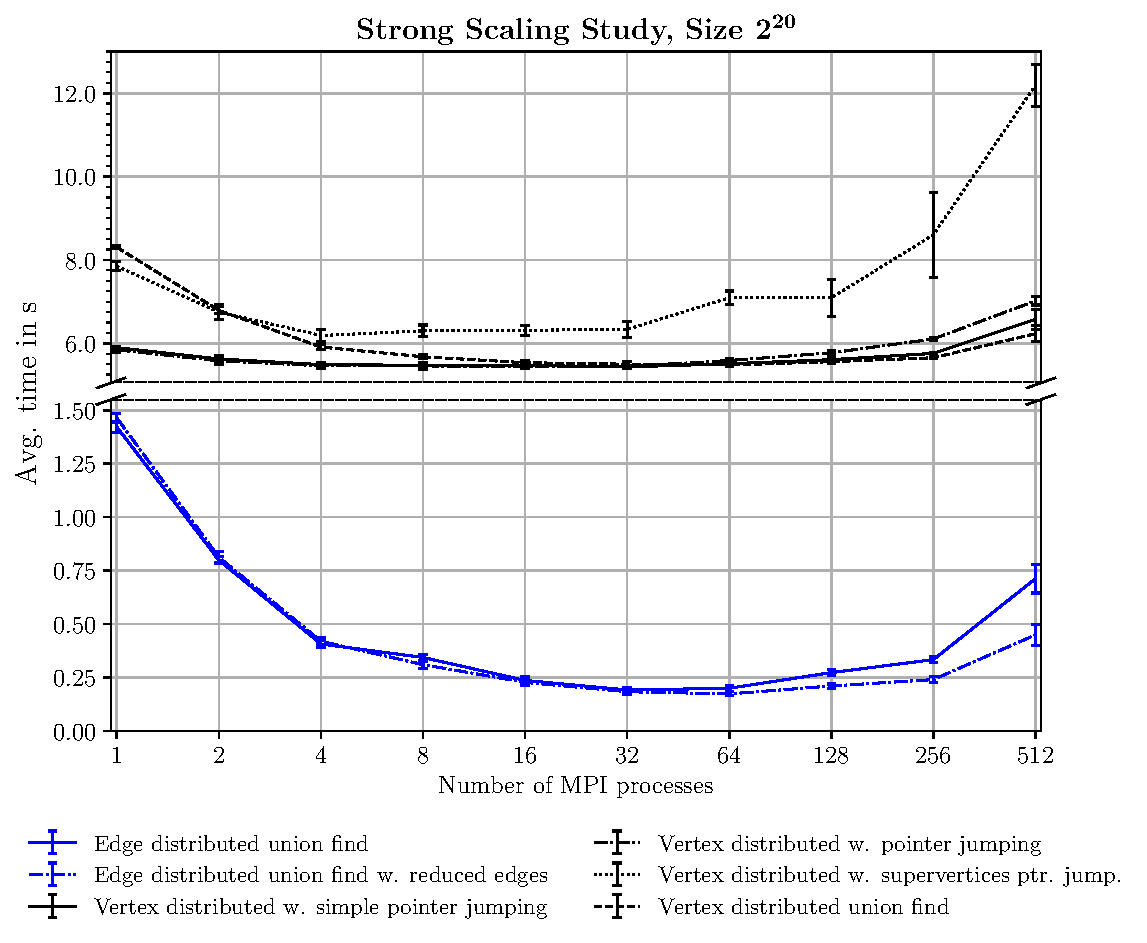
\includegraphics[width=\columnwidth]{../benchmark-results/plots/strongscaling_s20.pdf}
  \caption{Strong scaling comparison without the baseline, $2^{20}$ vertices}
  \label{fig:strongscaling-20}
\end{figure}

\begin{table}[!t]
	\centering
  \resizebox{0.75\columnwidth}{!}{
	\begin{tabular}{l l l}
		\toprule
		\textbf{MPI processes} & \textbf{Best impl.} & \textbf{Parallel BGL} \\ \midrule
		$1$ & $0.5050$ & $13.0532$\\ 
		$4$ & $0.2997$ & $9.4513$\\ 
		$8$ & $0.2001$ & $5.3956$\\
		$16$ & $0.1254$ & $3.4787$\\
		$32$ & $0.11$ & $2.6483$\\
		$64$ & $0.1085$ & $2.4329$\\
		$128$ & $0.1094$ & $2.4421$\\ \bottomrule
	\end{tabular}}
	\caption{Runtime results in seconds from strong scaling comparison, $2^{19}$ vertices}
	\label{tab:strongscaling-19-table}
\end{table}

\mypar{Baseline Comparison}
The results of the strong scaling comparison for the baseline comparison are presented in Fig.
\ref{fig:strongscaling-19}. All our implementations exceed the performance of Parallel BGL when work is distributed on
$8$ or fewer MPI processes. For more than $8$ MPI processes, only the edge distributed algorithms outperform the
baseline. We verified that these results are statistically significant by making sure that the $90\%$ confidence
intervals do not overlap. An interesting observation is that Parallel BGL performs exceptionally poorly for low MPI core
counts, whilst our implementations are more consistent. Table \ref{tab:strongscaling-19-table} contains the absolute
runtimes of our best implementation, \emph{Edge Distributed Union Find with reduced edges}, and the baseline. The best
speedup of $9.4513s/0.2997s \approx 31.5$ was achieved when using $2$ processes.

\begin{figure}
  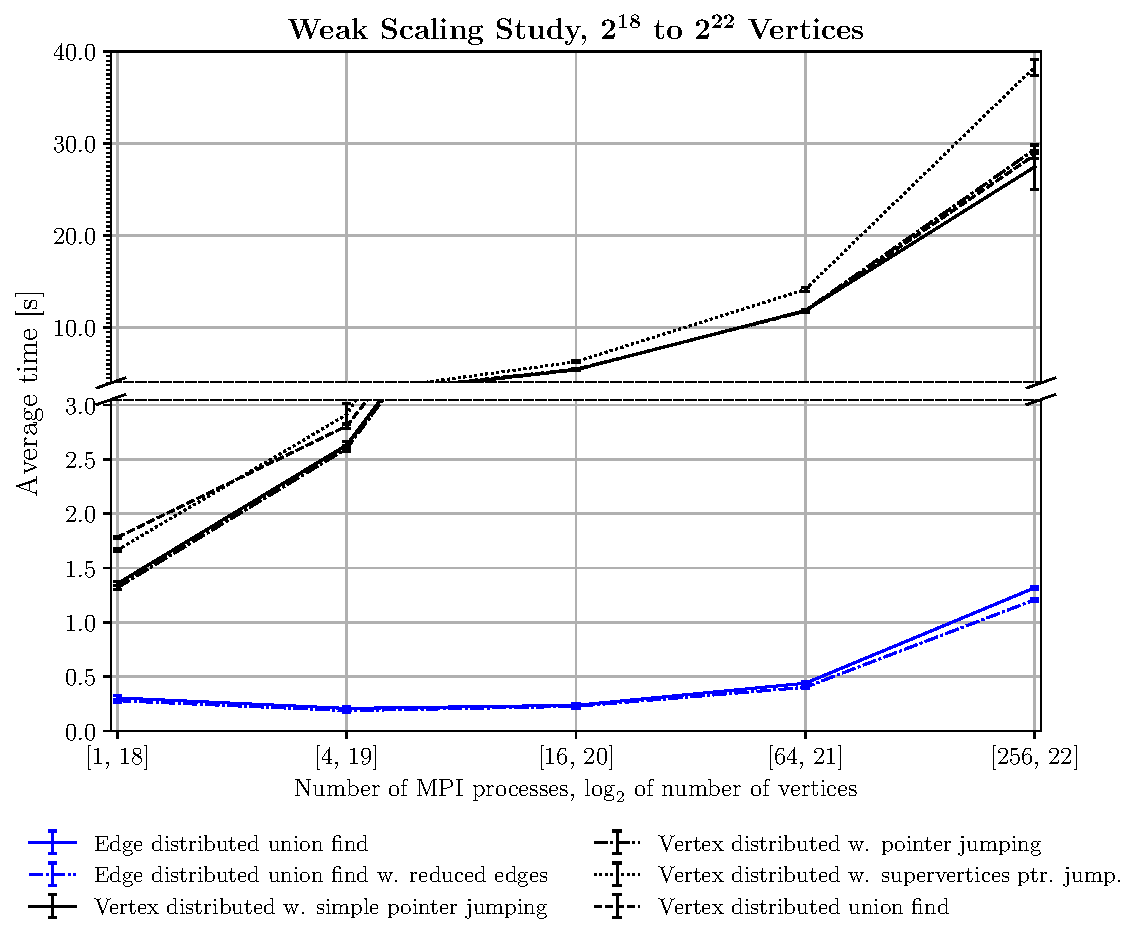
\includegraphics[width=\columnwidth]{../benchmark-results/plots/weakscaling.pdf}
  \caption{Weak scaling comparison, $2^{18}$ - $2^{22}$ vertices}
  \label{fig:weakscaling}
\end{figure}

\mypar{Implementation Comparison}
Fig. \ref{fig:strongscaling-20} contains the results of our strong scaling comparison. As can be seen, the edge
distributed implementations outperform the vertex distributed implementations substantially. All vertex distribution
implementation perform similarly apart from the supervertices pointer jumping one which performs worse in comparison as
the number of MPI processes increases. The reason for this is explained in the fine-grained analysis. It is also worth
mentioning, that the standard deviation for all implementations is minuscule, except the one of the supervertex pointer
jumping. This is most likely due to the randomness of that merging strategy. Another interesting point is that the edge
distributed implementations do not scale after reaching $16$ MPI processes. As the ratio between vertices and edges is
exactly $1:16$, it is not surprising to see diminishing returns past $16$ MPI processes. This is because the lightest
edge computation communicates proportionally to the amount of vertices of the input graph. After the $16$ process
threshold, the communication outweighs the per-process work, resulting in worse performance for increasing MPI
processes. More dense graphs might benefit from running on more MPI processes. The weak scaling comparison of Fig.
\ref{fig:weakscaling} shows a similar picture. In addition, the weak scaling comparison indicates that the edge
distributed implementations will perform better with a growing number of processes and increasing number of vertices.

\begin{figure}
  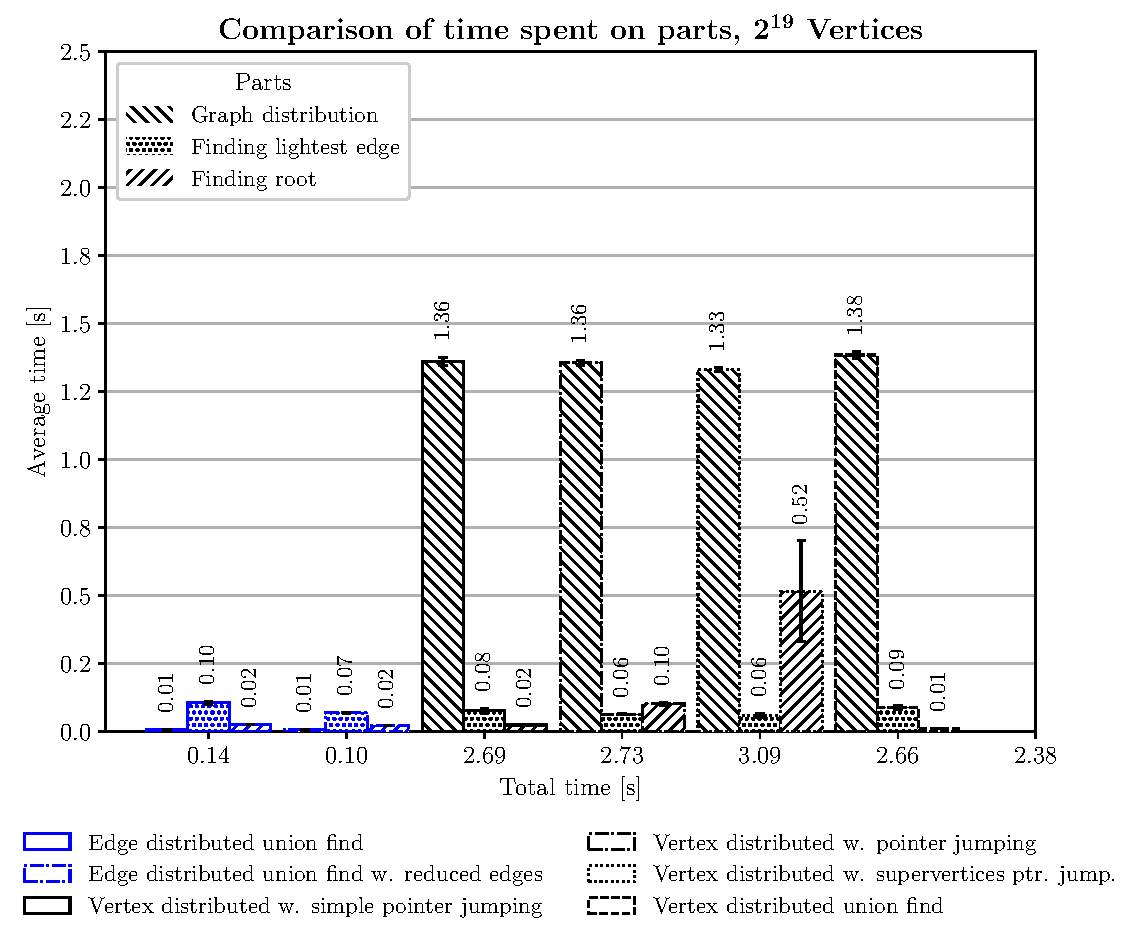
\includegraphics[width=\columnwidth]{../benchmark-results/plots/comparison.pdf}
  \caption{Comparison of time spent on parts, $2^{19}$ vertices, 64 MPI processes}
  \label{fig:comparison}
\end{figure}

\mypar{Detailed Runtime Analysis}
Fig. \ref{fig:comparison} gives a more detailed view and compares the runtime of the algorithm parts. The work
distribution is an immense bottleneck for the vertex distributed implementations, whereas it only makes up a small part
of the total runtime of the edge distributed implementations. An explanation of this could be, that the edge
distribution implementations use an \verb|MPI_Scatter|, potentially implemented as a tree. In the vertex distribution
implementations, the work is sequentially distributed by the MPI process \verb|0|. The lightest edge selection performs
very similarly across all implementations. On the other hand, the Union Find merging strategy outperforms all others,
except for the iterative vertex fixing approach. Interestingly, this approach outperforms the other two pointer jumping
strategies, even though it has a worse theoretical runtime. This result indicates that the additional synchronization
required is not worth the tighter theoretical runtime bound. The same holds for the supervertex pointer jumping, the
strategy requiring the most synchronizations, which performed poorly in the strong scaling comparison. In addition, the
plot shows that the large standard deviation of the \emph{Vertex Distributed Supervertex Pointer Jumping} implementation
comes from the merge step. This strengthens the claim made in the previous paragraph.

\section{Conclusions}
% Here you need to summarize what you did and why this is
% important. {\em Do not take the abstract} and put it in the past
% tense. Remember, now the reader has (hopefully) read the report, so it
% is a very different situation from the abstract. Try to highlight
% important results and say the things you really want to get across
% such as high-level statements (e.g., we believe that .... is the right
% approach to .... Even though we only considered x, the
% .... technique should be applicable ....)
As is evident from the benchmark evaluation in section \ref{sec:results}, we outperform the Parallel BGL by a wide
margin. The best approach to distribute the work is the edge distribution strategy. The merging strategy used by the algorithm does not have a significant impact on
the performance. However, the \emph{Supervertex Pointer Jumping} performs the worst. In conclusion, we can say that we
achieved our goal and found approaches that perform better than one state of the art implementation. The Parallel BGL
is, of course, more sophisticated and supports generic graph data structures as well as other algorithms. The results we
found are similar to those of Chung and Condon \cite{chung1996parallel} in that supervertex pointer jumping performs
worse than pointer jumping on structured and random graphs.

\mypar{Future Work}
% You can also formulate next steps if you want. Be brief. After the conclusions there are only the references.
Besides the obvious step of finding new strategies and implementing more combinations, a possible way on how to improve
the current implementations is by resolving the limitations described in section \ref{par:limitation}. In particular,
storing the actual MST and supporting all MPI configurations independent of the input graph. Moreover, depending on
graph properties, such as the connectivity or the average degree, different strategies could be applied at run-time.
This would require further, more-detailed measurements. Other work could also try to benchmark different graph types,
for instance Erdös-Renyi graphs, and figure out which graph properties influence the runtimes. Moreover, it would be
interesting to see if a parallelized merging strategy using a wait-free Union-Find data structure \cite{wfuf} performs
better than our current implementations.

% \section{Further comments}
%
% Here we provide some further tips.
%
% \mypar{Further general guidelines}
% 
% \begin{itemize}
% \item For short papers, to save space, I use paragraph titles instead of
% subsections, as shown in the introduction.
% 
% \item It is generally a good idea to break sections into such smaller
% units for readability and since it helps you to (visually) structure the story.
% 
% \item The above section titles should be adapted to more precisely
% reflect what you do.
% 
% \item Each section should be started with a very
% short summary of what the reader can expect in this section. Nothing
% more awkward as when the story starts and one does not know what the
% direction is or the goal.
% 
% \item Make sure you define every acronym you use, no matter how
% convinced you are the reader knows it.
% 
% \item Always spell-check before you submit (to us in this case).
% 
% \item Be picky. When writing a paper you should always strive for very
% high quality. Many people may read it and the quality makes a big difference.
% In this class, the quality is part of the grade.
% 
% \item Books helping you to write better: \cite{Higham:98} and \cite{Strunk:00}.
% 
% \item Conversion to pdf (latex users only): 
% 
% dvips -o conference.ps -t letter -Ppdf -G0 conference.dvi
% 
% and then
% 
% ps2pdf conference.ps
% \end{itemize}
% 
% \mypar{Graphics} For plots that are not images {\em never} generate the bitmap formats
% jpeg, gif, bmp, tif. Use eps, which means encapsulate postscript. It is
% scalable since it is a vector graphic description of your graph. E.g.,
% from Matlab, you can export to eps.
% 
% The format pdf is also fine for plots (you need pdflatex then), but only if the plot was never before in the format 
% jpeg, gif, bmp, tif.

\bibliographystyle{IEEEbib}
\bibliography{bibl_conf}

\end{document}

